\documentclass[final]{beamer}
%\usepackage{etex}

\usetheme{boxes}
\usecolortheme{rose}
\usefonttheme{professionalfonts}
%\setbeamertemplate{mini frames}{}
\usepackage[english]{babel}
\usepackage[utf8]{inputenc}
\usepackage[T1]{fontenc}
\usepackage{ae,aecompl}
\usepackage{amsfonts,amssymb,amsmath}
\usepackage{esint}
%\usepackage{epstopdf}
\usepackage{algorithmic}
% \usepackage{algorithm}
\usepackage{tikz}
\usetikzlibrary{arrows,shapes}
%\usepackage{xifthen}
\usepackage{pgfplots}
\usepackage{float}
\usepackage{ragged2e}
%\usepackage{latexsym}
%\usepackage[dvips]{pstricks} % PSTricks
%\usepackage{pst-node}
%\usepackage{psfrag}
%\usepackage{wrapfig}
%\usepackage{alltt}
%\usepackage{url}
%\usepackage{pict2e}
%\usepackage{multimedia}
%\usepackage{fancyvrb}
\usepackage{graphicx}
%\usepackage{verbatim}
%\usepackage{mathrsfs}
%\usepackage{multirow}
\usepackage{bm}
%\usepackage{algorithm2e}
\usepackage{hyperref}
%\usepackage[angle=0,scale=5,opacity=1,color=black]{background}
%\usepackage[active]{srcltx}
\usepackage{commath}
\usepackage{multicol}
\usepackage{subcaption}
\usepackage{siunitx}
%\usepackage[export]{adjustbox}

%\usetikzlibrary{spy}
%\tikzset{level 1 concept/.append style={font=\sf, sibling angle=60,level distance = 27mm}}
%\tikzset{level 2 concept/.append style={font=\sf, sibling angle=55,level distance = 17mm}}
%\tikzset{every node/.append style={scale=0.6}} 


%% Beamer Style Setup
%\definecolor{mywine}{rgb}{.5412,.0235,.0}
%\usecolortheme[named=mywine]{structure}
%\setbeamercolor{title}{fg=mywine}
%\setbeamercolor{frametitle}{fg=mywine}
%\setbeamercovered{transparent}
\setbeamertemplate{navigation symbols}{}

%% ALGORITHM Commands %%%%%%%%%%%%%%%%%%%%%%%%%%%%%%
\renewcommand{\algorithmicrequire}{\textbf{Input:}}
\renewcommand{\algorithmicensure}{\textbf{Output:}}
\newfloat{program}{thp}{Program}
\floatname{program}{}
\renewcommand*\theprogram{}
\newcommand{\theHalgorithm}{\arabic{algorithm}}
\newcommand{\eq}[1]{(\ref{#1})}




\newtheorem{remark}[theorem]{Remark}
\newtheorem{proposition}[theorem]{Proposition}


\renewcommand{\Im}{{\ensuremath{\mathrm{Im\,}}}}
\renewcommand{\Re}{{\ensuremath{\mathrm{Re\,}}}}

\newcommand{\R}{\mathbb{R}}
\newcommand{\C}{\mathbb{C}}
\newcommand{\N}{\mathbb{N}}

\setbeamertemplate{caption}[numbered]
\setbeamertemplate{bibliography item}{\insertbiblabel}

\selectlanguage{english}
\title[SIMP Optimization]{\bf Topological Optimization\\Using the SIMP Method}
\author[Mikal Nelson]{Mikal Nelson\\
Advisor: Paul Cazeaux
}
\institute[KU]{
{University of Kansas}\\
Department of Mathematics\\
mikal.nelson@ku.edu\\
}
\date[M.A. Thesis Defense]{
\small M.A. Thesis Defense\\
July 26\textsuperscript{th}, 2021
}
\titlegraphic{\hspace{0in}
\includegraphics[scale=0.35]{logos/ku_math_logo.png}\;

\includegraphics[scale=0.12]{logos/ku_logo}\;

}

\graphicspath{ {pictures/} }

\begin{document}

\begin{frame}
	\titlepage
\end{frame}

\begin{frame}{\textbf{Outline}}
	\begin{itemize}
		\item The Volume-to-Point (VP) Heat Conduction Problem
		\item The Heat Equation
		\item The Finite Volume Method (FVM)
		\begin{itemize}
			\item FVM Discretization of Heat Equation
		\end{itemize}
		\item Optimization
		\begin{itemize}
			\item The Method of Moving Asymptotes (MMA)
		\end{itemize}
		\item Solid Isotropic Material with Penalization (SIMP)
		\item Numerical Experiments
	\end{itemize}
\end{frame}

\begin{frame}[t]{The Volume-to-Point (VP) Heat Conduction Problem}
	\pause
	Consider a finite-size volume in which heat is being generated at \textit{every} point, and which is cooled through a small patch (the heat-sink) located on its boundary.
	\pause
	\vfill
	Suppose that we have a finite amount of high-conductivity ($k_+$) material available.
	\vfill
	\pause
	Our goal is to determine the optimal distribution of the $k_+$ material through the given volume such that \textit{the average temperature is minimized}.\vfill
\end{frame}

\begin{frame}
	\begin{figure}
		\centering
		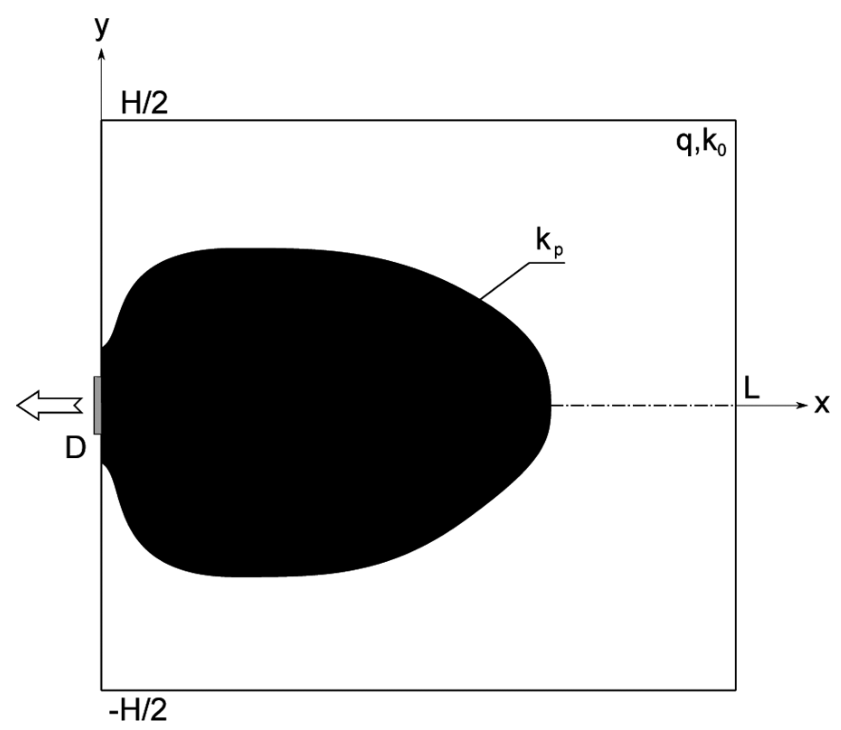
\includegraphics[height=0.65\textwidth]{VP-Problem.png}
		\caption[VP Problem Diagram]{Finite-size volume generating heat $(q, k_0)$ cooled thanks to a high-conductivity structure ($k_p$) with an arbitrary shape. \cite{Marck2012}}
	\end{figure}
\end{frame}

\begin{frame}
	\begin{figure}
		\centering
		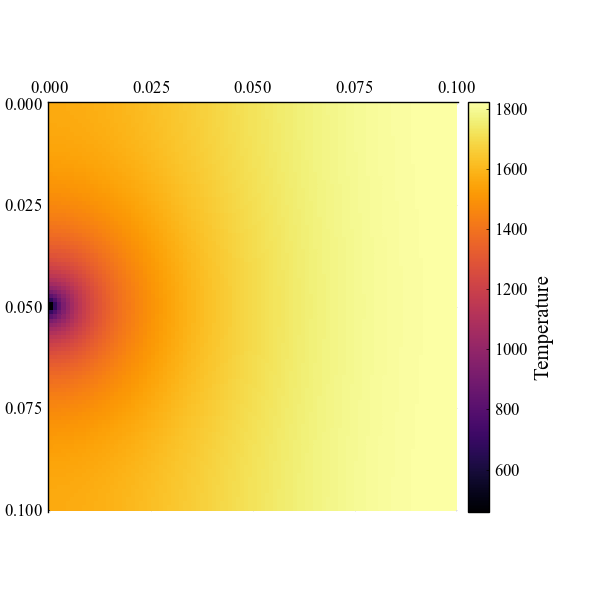
\includegraphics[height=0.65\textwidth]{Heatmap_Example.png}
		\caption[Heatmap Example]{Heatmap for a 0.1m $\times$ 0.1m object with uniform heat generation and a heat sink at the center of its west boundary. This map was produced via the Finite Volume Method using $100\times 100$ uniform control volumes.}
		\label{fig:heatmap-example}
	\end{figure}
\end{frame}

\begin{frame}{\textbf{The Heat Equation}}

The temperature ($T$) at any point in such an object is a function of both space ($\mathbf{x}$) and time ($t$) coordinates: $T(\mathbf{x},t)$.\\\vspace{1em}\pause
Physical principles demand that such a temperature function must satisfy the equation
\begin{equation}
	\frac{\partial T}{\partial t}=\nabla\cdot\left(k(\mathbf{x})\nabla T\right)\label{eqn:HeatEq},
\end{equation}
where $\nabla$ is the gradient operator and the function $k$ represents the thermal diffusivity at a point in our object.
\end{frame}

\begin{frame}[t]{\bf The Finite Volume Method (FVM)}
	To numerically solve the heat equation, we employ the Finite Volume Method (FVM).\pause
	\vfill
	Given a mesh of polygons (rectangles) on a domain $\Omega$ with sample points at $\lbrace x_i\rbrace\subset\Omega$, we create a set of \textit{control volumes} around each $x_i$. This set of control volumes will be used to discretize the partial differential equation.\\\vfill\pause
	The main idea of FVM is to integrate the heat equation over each control volume and then use the Divergence Theorem to convert volume integrals into surface integrals involving the fluxes across the boundaries of the control volumes.
	\vfill
\end{frame}

\begin{frame}[plain]
	\begin{theorem}[The Divergence Theorem]
		Suppose that $\mathcal{V}$ is a compact subset of $\mathbb{R}^n$ that has a piecewise smooth boundary $\mathcal{S}$ (i.e. $\partial\mathcal{V}=\mathcal{S}$) with outward pointing normal vectors. If $\mathbf{F}$ is a continously differentiable vector field defined on a neighborhood of $\mathcal{V}$, then
		\begin{equation}
			\iiint_{\mathcal{V}}\left(\nabla\cdot\mathbf{F}\right)\dif\mathcal{V}=\oiint_{\mathcal{S}}\left(\mathbf{F}\cdot\mathbf{\hat{n}}\right)\dif\mathcal{S}\label{eqn:div-thm}
		\end{equation}
		where $\hat{\mathbf{n}}$ is the outwards pointing normal vector to the boundary.
		\label{thm:div-thm}
	\end{theorem}
\end{frame}

\begin{frame}[t]{\bf Discretization of Heat Equation}
	\begin{equation}
		\int_{V_i}\frac{\partial T}{\partial t}\dif\mathbf{x}=\int_{V_i}\nabla\cdot \left(k(\mathbf{x})\nabla T\right)\dif\mathbf{x}\underset{\eqref{eqn:div-thm}}{=}\int_{\partial V_i}k(\mathbf{x})\nabla T\cdot\hat{\mathbf{n}}\dif s\label{eqn:Vol-to-Surface-FVM}
	\end{equation}\\
	\vspace{1em}
	\pause
	In a rectangular grid there are only four neighboring cells which we can label as North, South, East, West.\\\vspace{1em}
	\pause
	For a control volume $V_i$ we'll label the North boundary as $\partial V_N$, the South boundary as $\partial V_S$, the East boundary as $\partial V_E$, and the West boundary as $\partial V_W$.\\\vspace{1em}
	\pause
	Additionally, let $\Delta x$ be the length of the North and South boundaries, and $\Delta y$ the length of the East and West boundaries.
\end{frame}

\begin{frame}
	\begin{figure}
		\includegraphics[width=0.8\linewidth]{FVM-grid.png}
		\caption{Portion of two-dimensional grid using in the Finite Volume Method for a control volume $V_P$. \cite[p. 129]{Versteeg2007}}
	\end{figure}
\end{frame}

\begin{frame}[t]{\bf Discretization of Heat Equation}
	\begin{equation*}
		\int_{V_i}\frac{\partial T}{\partial t}\dif\mathbf{x}=\int_{V_i}\nabla\cdot \left(k(\mathbf{x})\nabla T\right)\dif\mathbf{x}\underset{\eqref{eqn:div-thm}}{=}\int_{\partial V_i}k(\mathbf{x})\nabla T\cdot\hat{\mathbf{n}}\dif s
	\end{equation*}
\vfill
\pause
Recognizing that $\partial V_i=\partial V_N\cup\partial V_S\cup\partial V_E\cup\partial V_W\ldots$
\vfill
\pause
	\hspace*{-2pt}\makebox[\linewidth][c]{%
	\begin{tabular}{ccc}
		$\displaystyle\int_{\partial V_i}k(\mathbf{x})\nabla T\cdot\hat{\mathbf{n}}\dif s$ & $=$ & $\displaystyle\int_{\partial V_N}k(\mathbf{x})\nabla T\cdot\hat{\mathbf{n}}_N\dif s+\int_{\partial V_S}k(\mathbf{x})\nabla T\cdot\hat{\mathbf{n}}_S\dif s$\\
		&  & $\displaystyle+\int_{\partial V_E}k(\mathbf{x})\nabla T\cdot\hat{\mathbf{n}}_E\dif s+\int_{\partial V_W}k(\mathbf{x})\nabla T\cdot\hat{\mathbf{n}}_W\dif s$
	\end{tabular}
	}
\vfill
\end{frame}

\begin{frame}[t]{\bf Discretization of Heat Equation}
	\hspace*{-2pt}\makebox[\linewidth][c]{%
		\begin{tabular}{ccc}
			$\displaystyle\int_{\partial V_i}k(\mathbf{x})\nabla T\cdot\hat{\mathbf{n}}\dif s$ & $=$ & $\displaystyle\int_{\partial V_N}k(\mathbf{x})\nabla T\cdot\hat{\mathbf{n}}_N\dif s+\int_{\partial V_S}k(\mathbf{x})\nabla T\cdot\hat{\mathbf{n}}_S\dif s$\\
			& & \\
			& & $\displaystyle+\int_{\partial V_E}k(\mathbf{x})\nabla T\cdot\hat{\mathbf{n}}_E\dif s+\int_{\partial V_W}k(\mathbf{x})\nabla T\cdot\hat{\mathbf{n}}_W\dif s$\\
			& & \\
			\pause
			$\displaystyle\int_{V_i}\frac{\partial T}{\partial t}\dif\mathbf{x}$ & $\approx$ & $\displaystyle k_N\frac{T_N-T_i}{\|\mathbf{x}_N-\mathbf{x}_i\|}\Delta x+k_S\frac{T_S-T_i}{\|\mathbf{x}_S-\mathbf{x}_i\|}\Delta x$\\
			& & \\
			& & $\displaystyle+k_E\frac{T_E-T_i}{\|\mathbf{x}_E-\mathbf{x}_i\|}\Delta y+k_W\frac{T_W-T_i}{\|\mathbf{x}_W-\mathbf{x}_i\|}\Delta y$\\
			& & \\
			\pause
			$\displaystyle\implies \Delta x\Delta y\frac{\dif T_i}{\dif t}$ & $=$ & $\displaystyle\left( k_N\frac{T_N-T_i}{\|\mathbf{x}_N-\mathbf{x}_i\|}+k_S\frac{T_S-T_i}{\|\mathbf{x}_S-\mathbf{x}_i\|}\right)\Delta x$\\
			& & \\
			& & $\displaystyle+\left(k_E\frac{T_E-T_i}{\|\mathbf{x}_E-\mathbf{x}_i\|}+k_W\frac{T_W-T_i}{\|\mathbf{x}_W-\mathbf{x}_i\|}\right)\Delta y$
		\end{tabular}\label{deriv:descrete-FVM}
	}
\end{frame}

\begin{frame}{\textbf{The Optimization Problem}}
	\pause
	\begin{definition}
		An optimization problem (in standard form) has the form
		\begin{equation}
			\begin{tabular}{lll}
				\text{minimize }   & $f_0(\mathbf{x})$        &                 \\
				\text{subject to } & $f_i(\mathbf{x})\leq 0$, & $i=1,\ldots, m$ \\
				& $h_i(\mathbf{x}) = 0$,   & $i=1,\ldots, p$ 
			\end{tabular}\label{Optimization}
		\end{equation}
		where
		\begin{itemize}
			\item $\mathbf{x}=\left(x_1,\ldots,x_n\right)$ are the optimization variables,
			\item $f_0 : \mathbb{R}^n\rightarrow\mathbb{R}$ is the objective function,
			\item $f_i : \mathbb{R}^n\rightarrow\mathbb{R}$ are the inequality constraint functions, and
			\item $h_i : \mathbb{R}^n\rightarrow\mathbb{R}$ are the equality constraint functions.
		\end{itemize}
	\end{definition}
	\pause
	In our VP problem we are concerned with minimizing the function $f_{av}(T)$, the average temperature, subject to an inequality constraint on the maximum volume of conductive material.
\end{frame}

\begin{frame}{\textbf{Optimization Methods}}
	Unconstrained optimizations algorithms follow a general blueprint:\pause
	\begin{enumerate}
		\item Choose an initial ``guess'' for the optimal value $x$\pause
		\item Find a descent direction $\Delta x$\pause
		\item Use a line search method to determine an appropriate step-size ($t$) in the descent direction\pause
		\item Compute new approximation value: $x+t\Delta x$\pause
	\end{enumerate}
	\pause
	\vfill
	The main differentiating factor between methods is how the descent direction is determined.\pause
	\vfill
	For example, the Gradient Descent algorithm chooses $\Delta x=-\nabla f(x)$ as the descent direction, while the Conjugate Gradient method requires that descent directions be conjugate to one another.
\end{frame}

\begin{frame}
	\begin{figure}
		\centering
		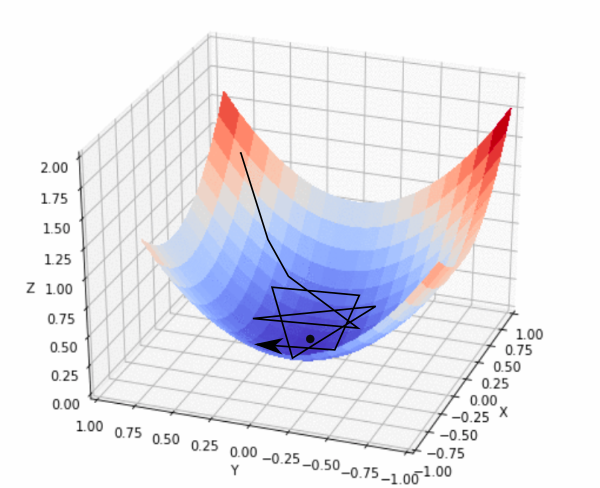
\includegraphics[height=0.75\textheight]{fastlr.png}
		\caption{A gradient descent algorithm in action. \cite{kathuria_2020}}
	\end{figure}
\end{frame}

\begin{frame}{}
	The VP problem is a \textit{constrained} optimization problem.\vfill\pause
	Additionally, it is not a convex problem.\vfill\pause
	(Convex problems have a lot of properties we can take advantage of that make the optimization problem easier to solve. Most notably, for a convex optimization problem, all local optima are global optima.)\vfill\pause
	Hence, we will employ a more complicated optimization algorithm.\vfill
\end{frame}

\begin{frame}[t]{\textbf{The Method of Moving Asymptotes (MMA)}}
	 The Method of Moving Asymptotes is a method of nonlinear programming, originally developed for structural optimization \cite{Svanberg1987}. MMA is designed for constrained optimization problems.
	 \vfill\pause
	 The method uses an iterative process which creates a convex subproblem that is solved in each iteration. Each of these subproblems is an approximation of the original problem with parameters that change the curvature of the approximation.
	 \vfill\pause
	 These parameters act as asymptotes for the subproblem and moving the asymptotes between iterations stablizes the convergence of the entire process.
\end{frame}

{\small
\begin{frame}[t]{\textbf{The Method of Moving Asymptotes (MMA)}}
	\begin{description}
		\item[\textbf{\underline{Step 0}:}] Choose a starting point $\mathbf{x}^{(0)}$, and let the iteration index $k=0$.
		\item[\textbf{\underline{Step 1}:}] Given an iterate $\mathbf{x}^{(k)}$, calculate $f_i(\mathbf{x}^{(k)})$ and the gradients $\nabla f_i(\mathbf{x}^{(k)})$ for $i=0,1,\ldots,m$.
		\item[\textbf{\underline{Step 2}:}] Generate a subproblem $P^{(k)}$ by replacing the functions $f_i$ by approximating functions $f_i^{(k)}$, based on calculations from Step 1.
		\item[\textbf{\underline{Step 3}:}] Solve $P^{(k)}$ and let the optimal solution of this subproblem be the next iteration point $\mathbf{x}^{(k+1)}$. Let $k=k+1$ and go to Step 1.
	\end{description}\pause
	Each $f_i^{(k)}$ is obtained by a linearization of $f_i$ in variables of the type $$\frac{1}{x_j-L_j}\quad\text{or}\quad\frac{1}{U_j-x_j}$$ dependent on the signs of the derivatives of $f_i$ at $\mathbf{x}^{(k)}$. The values of $L_j$ and $U_j$ are normally changed between iterations and are referred to as moving asymptotes.
\end{frame}
}

\begin{frame}{\textbf{The Method of Moving Asymptotes (MMA)}}
	Essentially the algorithm is creating \textit{convex} approximations to the objective and constraint functions: $$f_i^{(k)}(\mathbf{x})=r_i^{(k)}+\sum\limits_{j=1}^{n}\left(\frac{p_{ij}^{(k)}}{U_j^{(k)}-x_j}+\frac{q_{ij}^{(k)}}{x_j-L_j^{(k)}}\right)$$\vfill\pause
	\begin{center}
		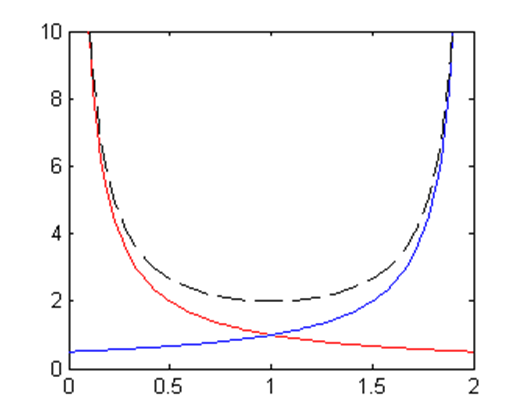
\includegraphics[width=0.4\linewidth]{MMA-pic.png}\cite{Keulen}
	\end{center}\pause
	These convex approximations can then be efficiently solved using methods such as gradient descent.\vfill\pause
	For our implementation of the SIMP method, the MMA algorithm was employed within the NLopt optimization package in Julia.\vfill
\end{frame}

\begin{frame}{\textbf{Solid Isotropic Material with Penalization (SIMP)}}
	Solid Isotropic Material with Penalization (SIMP) is a method based on topology optimization that can be used to solve the VP Heat Conduction Problem.\vfill\pause
	In each step of the SIMP method we increase or decrease the proportion of high-conductivity material used in our object by a small quantity.\\\vfill This allows us to apply methods designed for continuous optimization problems to the discrete VP problem as it transforms the binary 1---0 problem into a sequence of continuous problems.
\end{frame}

\begin{frame}{\textbf{Solid Isotropic Material with Penalization (SIMP})}
	\begin{figure}
		\begin{subfigure}{0.45\linewidth}
			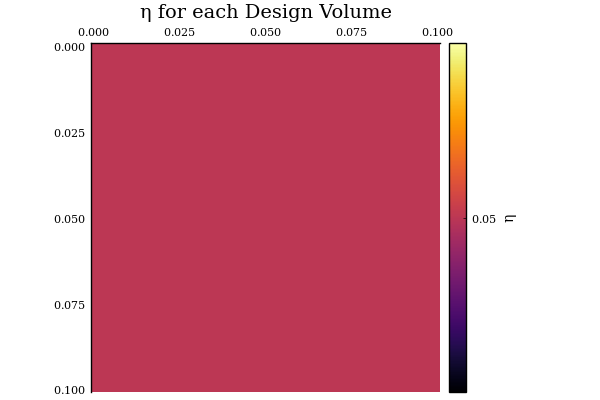
\includegraphics[width=\linewidth]{60x60-start-p=19-3iters.png}
			\caption{Initial Design}
		\end{subfigure}
		\begin{subfigure}{0.45\linewidth}
			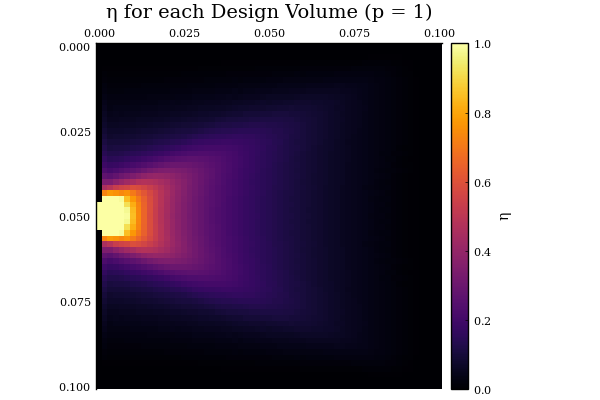
\includegraphics[width=\linewidth]{60x60_1p.png}
			\caption{Design After 1 Outer-Loop}
		\end{subfigure}
		\begin{subfigure}{0.45\linewidth}
			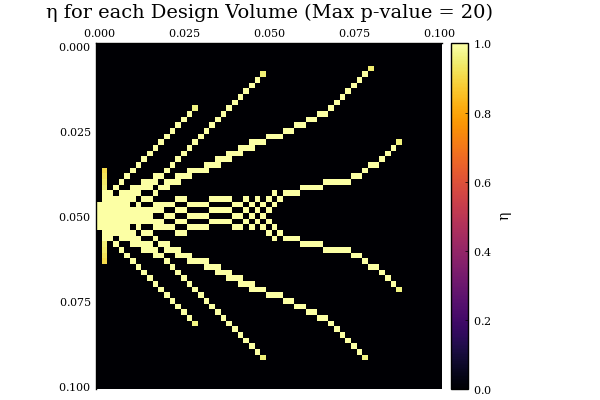
\includegraphics[width=\linewidth]{60x60-Final_Design.png}
			\caption{Final Design}
		\end{subfigure}
	\end{figure}
\end{frame}

{\footnotesize
\begin{frame}[t]{\textbf{Preliminary Parameters}}
	First of all, the energy differential equation driving the heat-flux inside the finite-volume requires:
	\begin{enumerate}
		\item All calculations are run under steady-state conditions. That is, we seek a stable solution where quantities are independent of time.
		\item All heat produced in the volume is evacuated through the heat sink.
		\item Low-conductivity materials ($k_0$) and high-conductivity materials ($k_+$) are treated as homogeneous and isotropic on their respective conductivities.
	\end{enumerate}\pause
	We also set the following conditions:
	\begin{itemize}
		\item Thermal conductivities depend only on the material, and therefore are constant:
		$$k_0=1 \si[per-mode=fraction]{\watt\per\square\meter\per\kelvin}\qquad\text{and}\qquad k_+=100 \si[per-mode=fraction]{\watt\per\square\meter\per\kelvin}$$
		\item All structures have a square aspect ratio with $L=H=0.1\si{\meter}$
		\item The heat-sink is located on the middle of the west side of the structure
		\item The heat-sink has Dirichlet boundary conditions: $T_S=0\si{\celsius}$
		\item All other boundaries are adiabatic (Neumann boundary conditions): $\nabla T\cdot\mathbf{n}=0$
	\end{itemize}
\end{frame}
}

\begin{frame}[t]{\textbf{Notation}}
	We use the following notation to describe the sets involved in the VP-problem:
	\begin{itemize}
		\item $\mathbf{x}\in\Omega$ = two-dimensional spatial field
		\item[] We set $\Omega = \Omega_0\cup\Omega_+$ where
		\begin{itemize}
			\item $\Omega_0$ = portion of $\Omega$ that has conductivity $k_0$.
			\item $\Omega_+$ = portion of $\Omega$ with conductivity $k_+$. This is the portion of the space with high-conductivity material.
		\end{itemize}
	\end{itemize}\vfill\pause
	Using the above established notation, we develop the following optimization problem:
	\begin{equation}
		\begin{tabular}{lll}
			\text{minimize }   & $f(T)$                                                   & \text{for } $\Omega_+$ \\
			\text{subject to } & $\nabla\cdot\left(k\nabla T\right)+q=0$  &                                      \\
			& $\mathbf{x}\in\Omega$ &                                      
		\end{tabular}\label{SIMP-Optimization-Problem}
	\end{equation}\vfill\pause
	The objective function $f(T)$ varies depending on desired design outcomes. Some possible objective functions include average temperature (used in our implementation), temperature variance, and maximum temperature.
\end{frame}

\begin{frame}{\textbf{Porosity Constraint}}
	We impose a constraint upon this problem to limit the quantity of $k_+$ material available:
	
	\begin{equation}
		\int_{\Omega_+}\dif\mathbf{x}=\int_{\Omega}\delta_+\dif\mathbf{x}\leq V\quad\text{where }\begin{cases}\delta_+ = 0 & \text{if }\mathbf{x}\in\Omega_0 \\ \delta_+ = 1 & \text{if }\mathbf{x}\in\Omega_+\end{cases}\label{eqn:vol-constraint}
	\end{equation}\vfill\pause
	Inequality \eqref{eqn:vol-constraint} imposes a cap on the maximum volume ($V$) of $\Omega_+$ and hence limits the available amount of high-conductivity material that can be applied to the domain.\vfill
	
	If we did not have this constraint, the optimal solution would be to set $\Omega_+=\Omega$, making the entire domain have high conductivity material.\vfill
\end{frame}

\begin{frame}{\textbf{Penalization Process}}
	The problem of whether to place high conductivity material in a particular location or not is discrete in nature. This is unfortunate as continuous optimization problems are generally easier to solve.\vfill\pause
	
	The SIMP method has a clever way of getting around this particular issue of discrete variables: create a continuous function that allows for a ``mix'' of the two conductive materials.\pause
	
	\begin{equation}
		k\left(\eta\right)=k_0+\left(k_+-k_0\right)\eta^p\qquad\text{with}\qquad 0\leq\eta\leq 1\qquad\text{and}\qquad p\geq1.\label{eqn:penalization}
	\end{equation}
	$\eta$ is called the \textit{design parameter} and $p$ the \textit{penalization parameter}.
\end{frame}

\begin{frame}[fragile]
	\begin{figure}
		\centering
		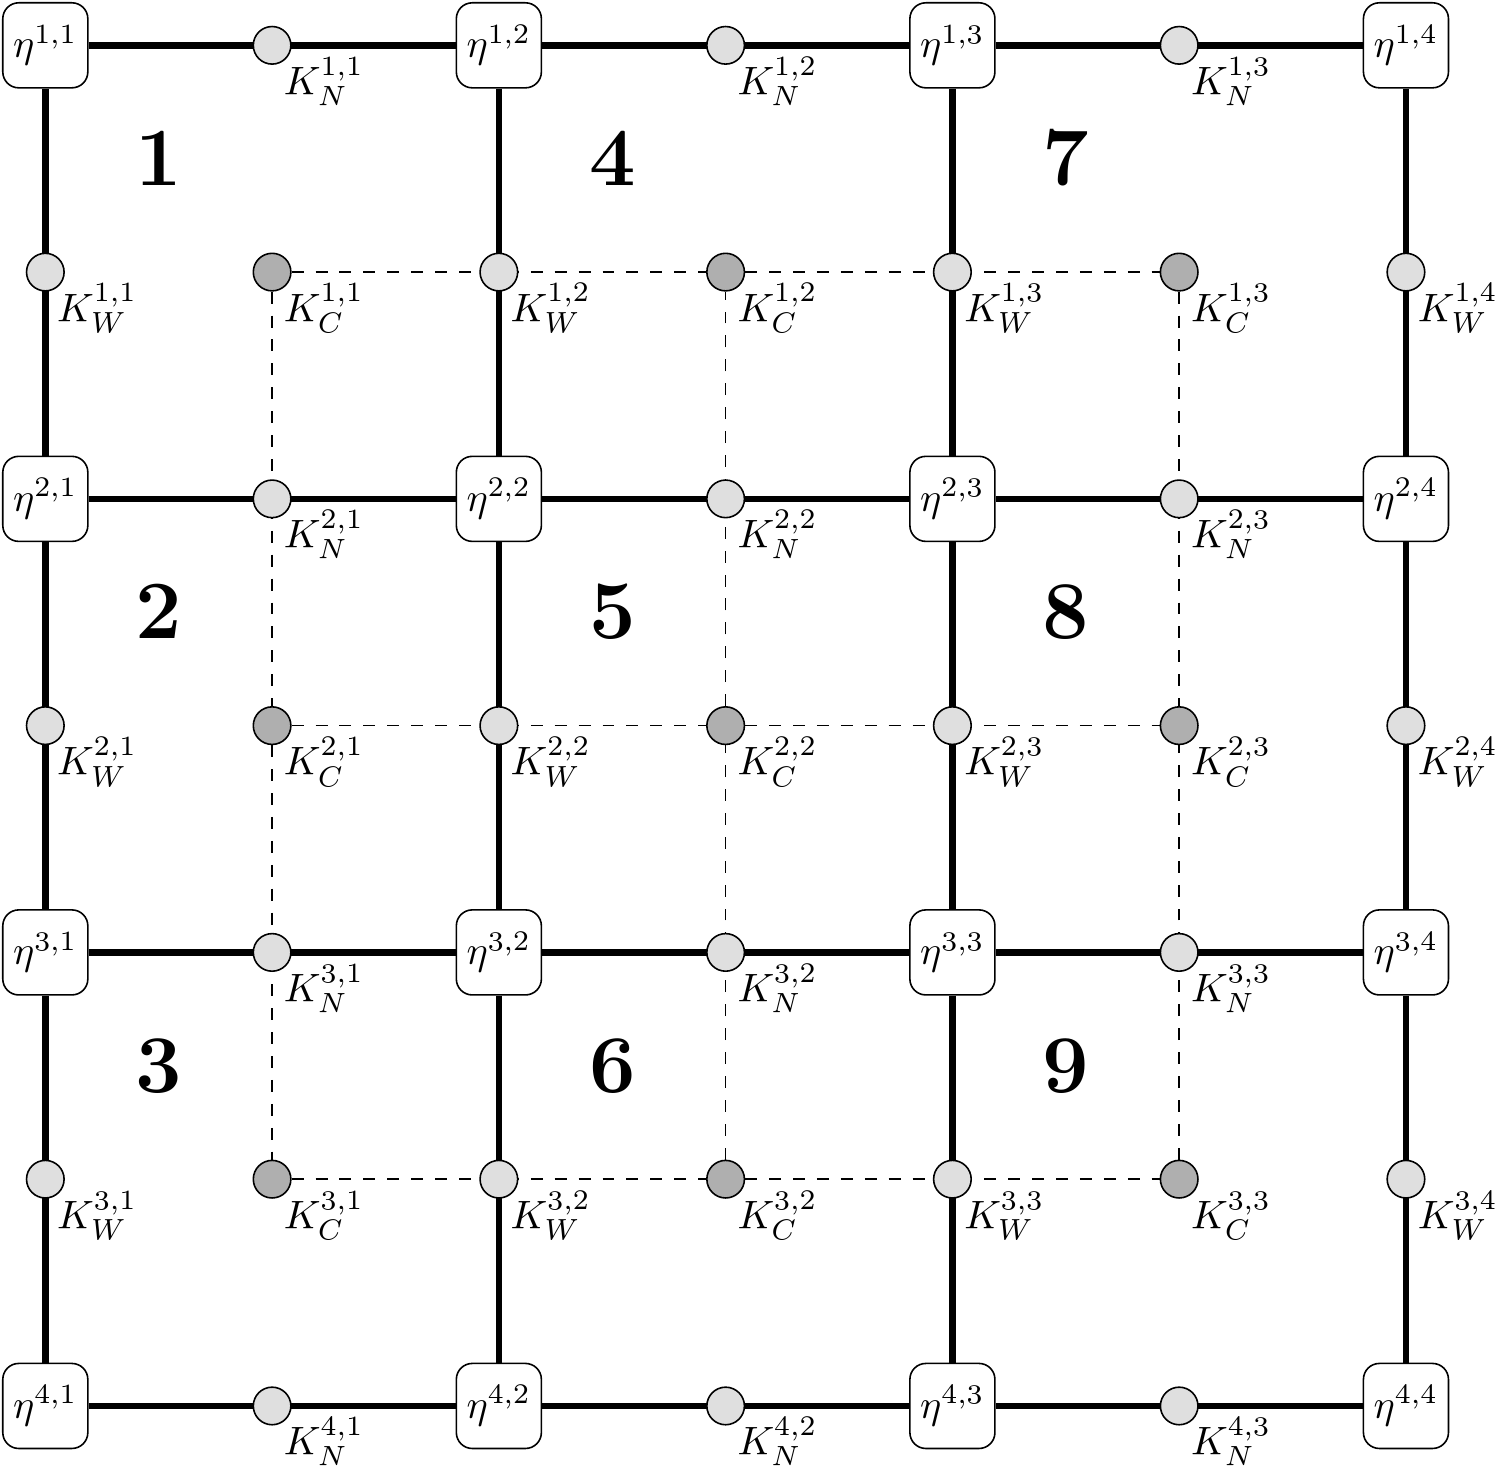
\includegraphics[height=0.75\textheight]{grid.png}
		\caption[Overlayed Design \& Temperature Grids]{\scriptsize Overlayed Temperature (\rule[0.55ex]{1.25em}{1.5pt}) and Design (\rule[0.6ex]{0.4em}{0.5pt}\,\rule[0.6ex]{0.4em}{0.5pt}\,\rule[0.6ex]{0.4em}{0.5pt}) grids with $4\times4$ Design Element $(\eta^{i,j})$ and $3\times3$ Temperature Control Volume $(K_C^{i,j})$ Nodes. $K_N^{i,j}$ and $K_W^{i,j}$ indicate nodes at the North and West boundaries, respectively, of each Temperature Control Volume. Each Temperature control volume is numbered beginning in the upper left and continuing column-by-column, left-to-right.}
		\label{fig:grids}
	\end{figure}
\end{frame}

\begin{frame}{\textbf{Discretization (Again!)}}
	\begin{equation}
		\nabla\cdot\left(k\nabla T\right)+q=0\label{eqn:SIMP-Heat-Eq}
	\end{equation}\pause
	For temperature control volume $(i,j)$, the finite volume method discretizes \eqref{eqn:SIMP-Heat-Eq} into the following linear equation
	{\small
		\begin{equation}
			K^{i,j}_C T^{i,j}=K_W^{i,j}T^{i,j-1}+K_W^{i,j+1}T^{i,j+1}+K_N^{i,j}T^{i-1,j}+K_N^{i+1,j}T^{i+1,j}+\Delta x\Delta y Q^{i,j}\label{eqn:FVM-Discret}
		\end{equation}}\pause
	The $K_W$ and $K_N$ coefficients are dependent on the thermal conductivity and cross-sectional area of their corresponding faces:
	\begin{equation}
		K_W^{i,j}=\frac{k_W^{i,j}\Delta y}{\Delta x}\qquad\text{and}\qquad K_N^{i,j}=\frac{k_N^{i,j}\Delta x}{\Delta y}\label{eqn:K-Coeffs}
	\end{equation}
	\begin{equation}
		k^{i,j}_W=\frac{k^{i,j}+k^{i+1,j}}{2}\qquad k^{i,j}_N=\frac{k^{i,j}+k^{i,j+1}}{2}
	\end{equation}\pause
	\begin{equation}
		K^{i,j}_C=K_W^{i,j}+K_W^{i,j+1}+K_N^{i,j}+K_N^{i+1,j}\label{eqn:CenterFluxCoeff}
	\end{equation}
\end{frame}

\begin{frame}{\textbf{Discretized Optimization Problem}}
	\begin{equation}
		\mathbf{K}\mathbf{T}=\Delta x\Delta y\mathbf{Q}.\label{eqn:KTQ-Matrix-Eqn}
	\end{equation}\pause
	Rearranging what we have done into matrix equations, we can get the following discretized formulation of the average temperature optimization problem:
	\begin{equation}
		\begin{tabular}{ll}
			$\text{minimize}$  & $f_{av}\left({\mathbf{T}}\right)=\frac{1}{N_T}\mathbf{1}^T\mathbf{T}$                                                                                     \\
			\text{subject to } & $\mathbf{K}\mathbf{T}=\Delta x\Delta y\mathbf{Q}$                                                                   \\
			& $\mathbf{1}^T\boldsymbol{\eta}-N_T\overline{\phi}\leq0$ \\
			& $\mathbf{k}=k_0\mathbf{1}+(k_+-k_0)\boldsymbol{\eta}^p$                                       \\
			& $0\leq\boldsymbol{\eta}\leq 1\text{ and } p\geq 1$
		\end{tabular}\label{Implementation-SIMP-Optimization-Problem}
	\end{equation}
	where $N_T$ represents the number of temperature control volumes and $\overline{\phi}$ represents the maximum porosity (the cap on the amount of high-conductivity material).
\end{frame}

\begin{frame}{\textbf{Numerical Experiments}}
	\begin{figure}
		\begin{subfigure}{0.4\textwidth}
			\centering
			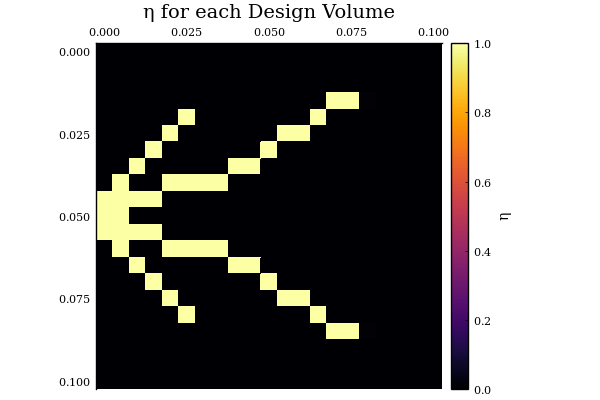
\includegraphics[width=1.1\linewidth]{20x20-Final_Design.png}
			\caption{$20\times 20$ control volumes}
			\label{fig:SIMP-Output-20}
		\end{subfigure}
		\begin{subfigure}{0.4\textwidth}
			\centering
			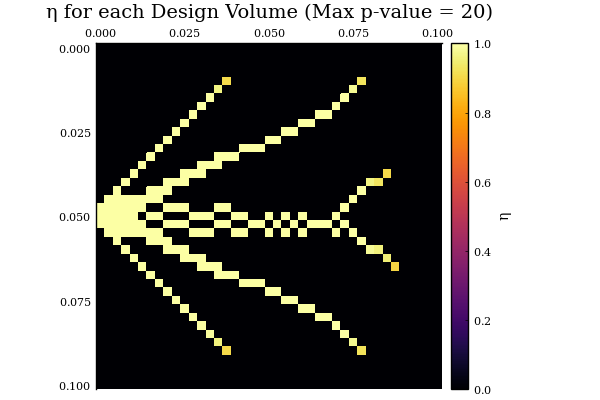
\includegraphics[width=1.1\linewidth]{40x40-Final_Design.png}
			\caption{$40\times 40$ control volumes}
			\label{fig:SIMP-Output-40}
		\end{subfigure}
		\begin{center}
			\begin{subfigure}{0.5\textwidth}
				\centering
				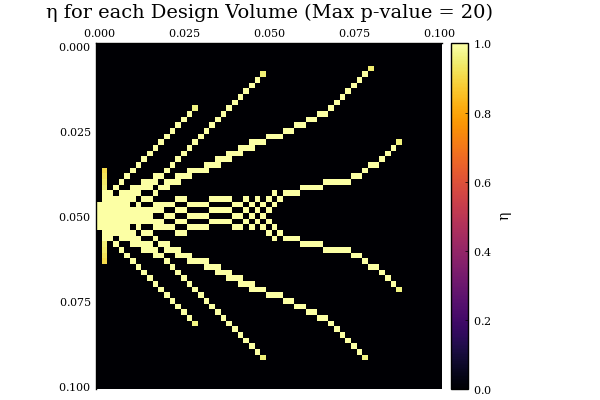
\includegraphics[width=\linewidth]{60x60-Final_Design.png}
				\caption{$60\times 60$ control volumes}
				\label{fig:SIMP-Output-60}
			\end{subfigure}
		\end{center}
	\end{figure}
\end{frame}

\begin{frame}{\textbf{Non-Square Grids}}
	\begin{figure}
		\begin{subfigure}{0.45\textwidth}
			\centering
			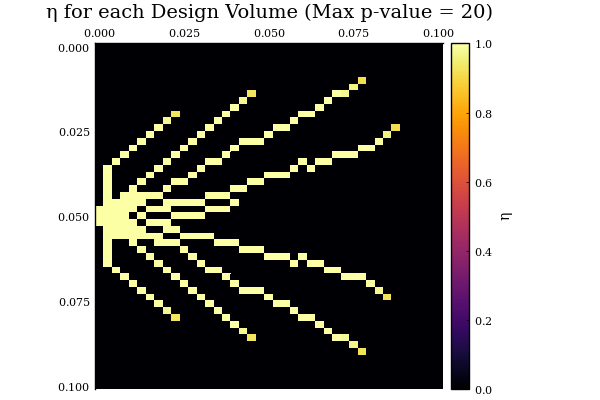
\includegraphics[width=1.1\linewidth]{50x40-Final_Design.png}
			\caption[Rectangular Control Volume Design]{$50\times 40$ control volumes}\label{fig:SIMP-Output-50-40}
		\end{subfigure}
		\begin{subfigure}{0.45\textwidth}
			\centering
			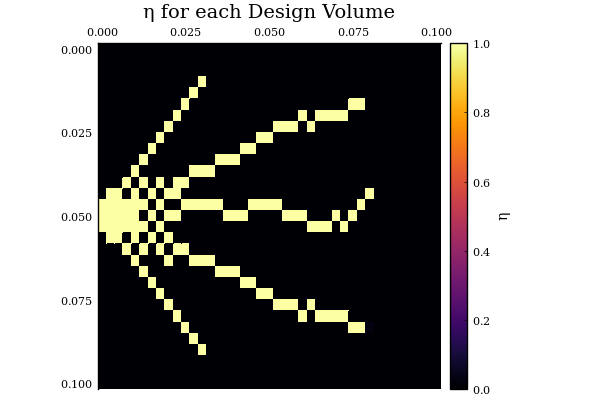
\includegraphics[width=1.1\textwidth]{SIMP-Example-Checkerboarding.png}
			\caption[Checkerboard Result in Practice]{$30\times 40$ control volumes}
			\label{fig:SIMP-Checkerboard}
		\end{subfigure}
	\end{figure}
\end{frame}

\begin{frame}{\textbf{Higher Initial Penalization}}
	\begin{figure}
		\begin{subfigure}{0.45\textwidth}
			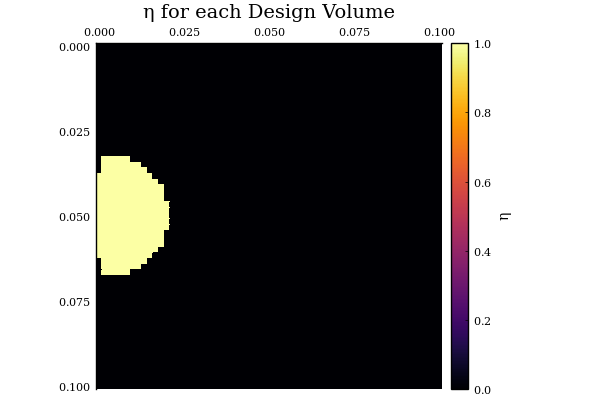
\includegraphics[width=1.1\linewidth]{60x60-start-p=5-1iters.png}
			\caption{$60\times 60$ Control Volumes with Initial $p=5$.}
			\label{fig:start_p=5}
		\end{subfigure}
		\begin{subfigure}{0.45\textwidth}
			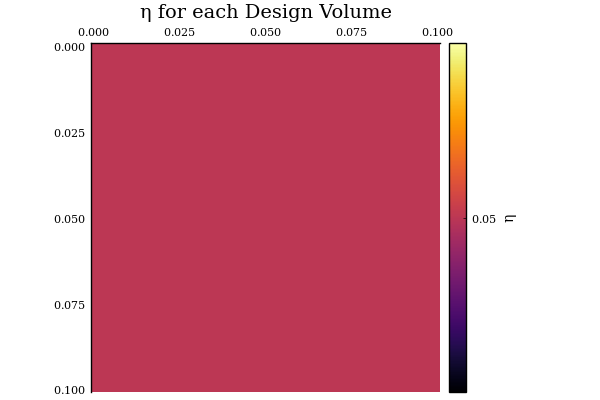
\includegraphics[width=1.1\linewidth]{60x60-start-p=19-3iters.png}
			\caption{$60\times 60$ Control Volumes with Initial $p=19$.}
			\label{fig:start_p=19}
		\end{subfigure}
		\caption[Designs with Higher Initial $p$]{Design outputs for initial $p$-values greater than $1$.}
	\end{figure}
\end{frame}

\begin{frame}{\textbf{Minimum Average Temperature Convergence}}
	\begin{figure}
		\centering
		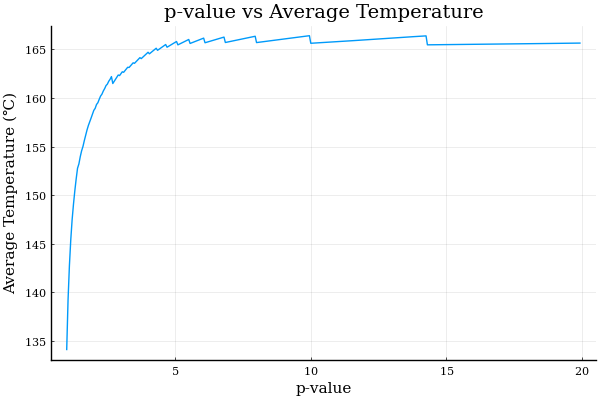
\includegraphics[width=0.9\linewidth]{60x60-p_vs_T.png}
		\caption[$p$-value vs. $T_{av}$]{$p$-value plotted against Average Temperature Evaluation for $60\times 60$ control volumes with a maximum $p$-value of $20$.}
		\label{fig:p-vs-T}
	\end{figure}
\end{frame}

\begin{frame}
	\begin{figure}
			\begin{subfigure}{0.45\textwidth}
				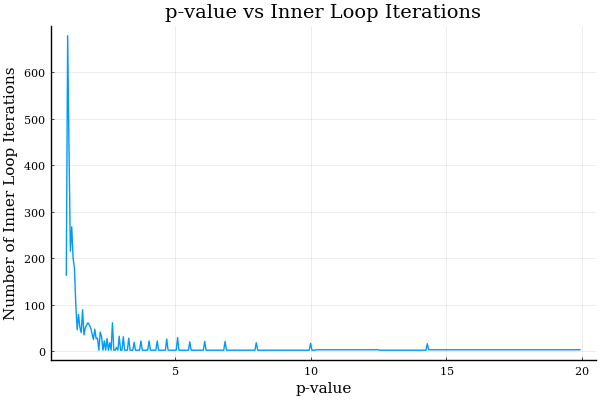
\includegraphics[width=\linewidth]{60x60-p_vs_Inner-Itter.png}
				\caption[$p$-value vs. $T_{av}$]{$p$-value plotted against the number of inner loop iterations for $60\times 60$ control volumes with a maximum $p$-value of $20$.}
				\label{fig:p-vs-Inner-Itter-60x60}
			\end{subfigure}
			\begin{subfigure}{0.45\textwidth}
				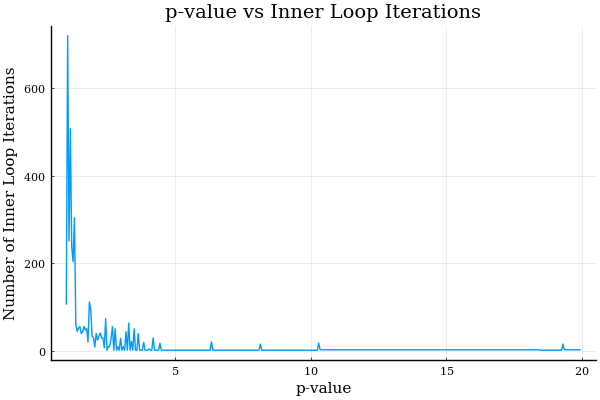
\includegraphics[width=\linewidth]{50x40-p_vs_Inner-Itter.png}
				\caption[$p$-value vs. $T_{av}$]{$p$-value plotted against the number of inner loop iterations for $50\times 40$ control volumes with a maximum $p$-value of $20$.}
				\label{fig:p-vs-Inner-Itter-50x40}
			\end{subfigure}
		\caption[$p$-value vs. Number of Inner Loop Iterations]{$p$-value vs. Number of Inner Loop Iterations for Square and Rectangular Control Volumes}
		\label{fig:p-vs-Inner-Itter}
	\end{figure}
\end{frame}

\begin{frame}{\textbf{Algorithm Runtime}}
	\begin{figure}
		\centering
		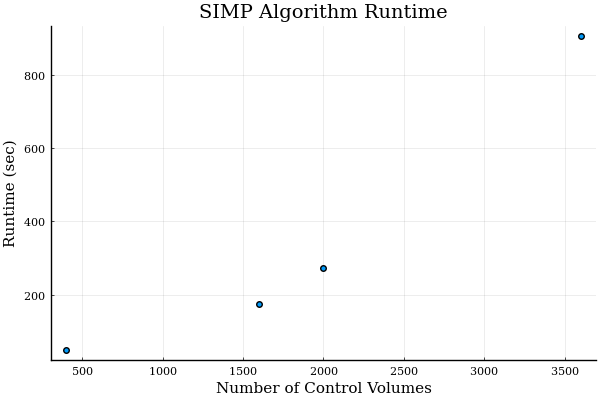
\includegraphics[width=0.8\linewidth]{SIMP-Runtime.png}
		\caption[SIMP Runtime Plot]{Plot of runtime for SIMP algorithm for various numbers of control volumes.}
		\label{fig:runtime}
	\end{figure}
\end{frame}

\frame[plain,allowframebreaks]{
\structure{\bf Bibliography}

\medskip
\begin{tiny}
\bibliographystyle{plain}
\bibliography{Thesis_Bibliography.bib}
\nocite{Boyd2004}
\nocite{Gander2018}
\nocite{kathuria_2020}
\nocite{Keulen}
\nocite{Marck2012}
\nocite{Svanberg1987}
\nocite{Versteeg2007}
\end{tiny}
}

\begin{frame}{\textbf{Questions?}}
	\begin{figure}
		\centering
		
\includegraphics[height=0.8\textheight]{elske.jpg}
	\end{figure}
\end{frame}

\end{document}